\chapter{Noise Robustness Across Molecular Representations and Model Architectures}\label{chap:robustness}
% TODO: Chapter 3 update pending. When it lands, search for `TODO: Ch3 update' in Chapters 1, 4 and 7 and re-check each quoted result. Also re-check the Chapter 3 Additional files and the abstract.
% [notes moved to thesis_notes_moved.md]

% TODO: review, needs manual review
% [CODE INPUT: commented out -- the Chapter 3 paper was not submitted, so it is not referenced]
% \textit{Preamble.} The work in this chapter is adapted from Punt, A., Hanser, T., Werner, S., and Morris, G.M., in preparation for the \textit{Journal of Cheminformatics}. Most of the figures, tables, and text in this chapter are therefore either identical or similar to the content of that manuscript. A signed Statement of Authorship for this jointly authored work is included in the front matter.

\section{Introduction}
% [notes moved to thesis_notes_moved.md]


% TODO: review, needs manual review
While there have been many investigations into the effect of noise on molecular property prediction, direct comparisons of how different molecular representations respond to label noise remain limited. The choice of molecular representation affects predictive performance. \citet{Deng2023} evaluated 62,820 models and found that ECFPs frequently outperform learned graph embeddings across models. This chapter asks whether these conclusions carry over to noise robustness. Between different types of label noise, \citet{Heid2023} found no difference in model performance between error distributions with the same mean and standard deviation. We expand on this by considering alternative patterns of noise, namely noise concentrated on a sparse subset of molecules or within scaffold families, an offset shared within each scaffold family, and labels clipped at an assay limit.

% TODO: review, needs manual review
This chapter addresses the four questions set out in Chapter~\ref{chap:intro}, namely how representation and model architecture divide the variance in predictive performance and in noise robustness, what probabilistic models add, whether the type of label noise matters, and whether uncertainty estimates track label noise.

\section{Methods}\label{sec:robustness:methods}
% ---- NOTES: Methods ----
% Takeaway: the study crosses four datasets, six representations, 20 model configurations, seven noise conditions and seven noise levels.
% Paragraph 1 (only if the section gets a lead-in paragraph):
% - Four datasets: QM9 (HOMO--LUMO gap) and three assay datasets (logD, Caco-2, hERG K$_i$).
% - Six representations, 20 model configurations, seven noise conditions, seven noise levels.
% - The 20 configurations are thirteen base models and seven variant models. Name both terms here; the Models subsection defines them.
% - The noise conditions are defined in Section~\ref{sec:noise_injection}. Hyperparameters are in Additional file~\ref{app:noise:sec:hyperparameters_default}.
% ---- END NOTES ----

% CODE INPUT
% TODO: check the count of variant models. The Chapter 3 results and Additional files name six variant models on the three assay datasets (19 models ranked there), while an earlier version of this paragraph said seven (20 configurations); the paragraph now says six, following paper.tex, whose six are RF (300 trees), GP (het.), the two BNNs with a variance head and the two heteroscedastic VBLL networks. The seventh is probably the Tanimoto-kernel GP, run on ECFP4 only; not verified which count holds on QM9.
% Checked 2026-09-30: the seventh is the Tanimoto-kernel GP (`gauche`). qsar_qm_models/scripts/figlib_config.py:580-594 puts it in VARIANT_MODELS and drops it from every cross-model figure and table (RERUN_PLAN.md 14.11v); results/decisions_arc_20260916/auc_norm_assay.csv and results/decisions_arc/auc_norm_qm9.csv hold it on ECFP4 only, on all four datasets, under three noise conditions. Six is the count of variant models that are reported.
% TODO: review, needs manual review
We used four datasets, namely QM9 with the HOMO--LUMO gap as the prediction target and three assay datasets for LogD, Caco-2 and hERG $K_i$. On each dataset we paired six representations with thirteen base models and six variant models, which the Models subsection describes. Every pairing was run under Gaussian, grouped-wider and grouped-shifted noise at seven noise levels, and the other four noise conditions (Section~\ref{sec:noise_injection}) were run on selected pairings. The hyperparameters of every model are given in Additional file~\ref{app:noise:sec:hyperparameters_default}.



\subsection{Datasets}

Although we are investigating the effects of label noise stemming from experimental settings, for the purposes of testing we inject controlled amounts of artificial noise into clean labels. Data were extracted from the QM9 molecular property dataset distributed by PyTorch Geometric \citep{Ramakrishnan2014}, which contains 130,831 small organic molecules with pre-computed quantum-mechanical properties obtained from density functional theory calculations at the B3LYP/6-31G(2df,p) level of theory. We selected the HOMO--LUMO gap as the prediction target in QM9, as it captures a molecule's electronic excitability, charge transfer capability, and chemical stability \citep{Fediai2023}. We assumed that QM9 labels were free of noise, notwithstanding approximations in the level of theory. Each experiment was replicated 10 times with a distinct random seed and a randomly selected subset of $N = 10{,}000$ molecules, split 80/10/10 into 8,000 training, 1,000 validation and 1,000 test molecules. All models were fitted on those 8,000 training molecules, except the Gaussian processes, which were fitted on a random subset of 5,000 of them; the validation and test molecules were unchanged.

We repeated these experiments on three molecular property datasets with experimentally determined endpoints. From the OpenADMET initiative \citep{openadmet}, we used LogD and Caco-2 efflux permeability, with $N = 5{,}039$ and $N = 2{,}161$ respectively. We also selected hERG $K_i$ data from ChEMBL \citep{Zdrazil2023}, following a protocol inspired by \citet{landrum2024}: filter for binding assays, deduplicate by median pChEMBL value, and remove compounds with an inter-assay standard deviation greater than 1.0 log unit, resulting in $N = 1{,}415$ compounds. Each of the three was partitioned into five folds by grouped $k$-fold cross-validation, and each fold's training block gave up a further grouped fifth as a validation set for early stopping. A model therefore fits between 3,194 and 3,364 of the 5,039 LogD molecules, depending on the fold, so the Gaussian-process subsample never applies to these datasets. Unlike QM9's 10 replicates, which are 10 independent draws from one pool, each assay dataset is a single fixed set in which every molecule is tested exactly once and nothing is redrawn.

All splits and cross-validation folds were grouped by the chirality-blind Bemis--Murcko scaffold, implemented such that each distinct acyclic molecule forms its own group, and groups are filled in random order. Prior to modeling, all molecular structures were sanitized and canonicalized using \texttt{RDKit} to remove invalid valence states and standardize atom and bond typing \citep{rdkit}. Prediction targets were standardized to zero mean and unit variance. Experiments that track uncertainty were run once rather than in replicates.

\subsection{Representations}

In this chapter, we evaluated six molecular representations: ECFP4, Avalon, Sort \& Slice, PDV, ChemBERTa and Molecular Hypergraph Grammar GNNs (MHG-GNNs). The same six were used on QM9 and on the three assay datasets. ECFP4 is a Morgan fingerprint with radius $r = 2$ with $d = 2048$ bits \citep{rogers2010, rdkit}. Sort \& Slice takes the same substructures as ECFP4, but it ranks them by prevalence and selects the top $L$ ($L=1024$) \citep{sns}. We fitted the Sort \& Slice vocabulary on the training molecules alone, refitting it for each QM9 replicate and for each cross-validation fold.  Avalon is a 2,048-bit fingerprint, generated with the Avalon toolkit through RDKit \citep{avalon, rdkit}. The PDV representation is a vector of 200 physicochemical descriptors computed with RDKit's \texttt{MolecularDescriptorCalculator} \citep{rdkit, Cherkasov2014}; the 200 are listed in Additional file~\ref{app:noise:sec:pdv_descriptors}, and the list is fixed in our code rather than taken from RDKit's default descriptor set, which grows between releases. ChemBERTa embeddings are the mean over the non-padding token embeddings of the \texttt{DeepChem/ChemBERTa-77M-MTR} checkpoint, producing 384 features \citep{Ahmad2022}. MHG-GNNs are a GIN-based autoencoder pre-trained on 1.34 million PubChem molecules using a $\beta$-variational autoencoder loss, producing 1,024-dimensional embeddings through iterative message passing and found in the published \texttt{mhggnn\_pretrained\_model\_0724\_2023} checkpoint \citep{kishimoto2023}. We z-score normalized PDV, ChemBERTa and MHG-GNN per feature, using the training molecules' mean and standard deviation; ECFP4, Avalon and Sort \& Slice reach the model as built.

\subsection{Models}
% [notes moved to thesis_notes_moved.md]

To understand model behavior in the presence of label noise, we explored a range of model types (Chapter~\ref{chap:background}). We fitted tree ensembles, a support vector machine, Gaussian processes and neural networks. Several are variants of one another, differing in the probabilistic machinery they add, and Additional file~\ref{app:noise:sec:hyperparameters_default} gives every configuration with its settings.

% TODO: review, needs manual review
Among the tree ensembles, we used RFs and QRFs. While we used 100 trees for RF, we observed a noisy quantile estimate with 100 trees for QRF, prompting us to use 300 instead. To observe the effect of the quantile mechanism, we then fit a second RF at 300 trees so the two models were identical in all other settings.

% TODO: review, needs manual review
We also used XGBoost, LightGBM and NGBoost. NGBoost uses validation data for early stopping. On QM9 this is the validation split. On the three assay datasets NGBoost receives the training molecules without the validation set, and holds out a scaffold-grouped fifth of them for early stopping.

% TODO: review, needs manual review
For the SVM, we used a radial basis function (RBF) kernel with $\gamma = \texttt{scale}$ and $C = 1.0$.

% TODO: review, needs manual review
We fitted three variants of GPs, each with a constant mean and a scaled kernel. The first uses an RBF kernel and runs on all six representations. The second uses the Tanimoto kernel \citep{Ralaivola2005, moss2020}, which is defined only on binary vectors, so it was run on ECFP4 alone, on all four datasets under Gaussian, grouped-wider and grouped-shifted noise. Because it covers only one of the six representations, it is not counted among the base or variant models, and its results are not reported in this chapter. The third is a heteroscedastic variant in which the RBF process is given a second network that predicts the observation noise of each molecule. Because the cost of an exact GP grows with the cube of the number of training molecules (Chapter~\ref{chap:background}), and sparse approximations introduce approximation error and can be harder to tune \citep{quinonero2005}, we used an exact GP and fit it on at most $5{,}000$ training molecules, drawn by a seeded sample. We implemented these GP models in \texttt{GPyTorch} \citep{gpytorch}, with the Tanimoto kernel taken from the \texttt{Gauche} framework \citep{gauche}.

We tested two deterministic feed-forward architectures, both fully connected and both implemented in PyTorch \citep{Paszke2019}: (i) NN-$\alpha$ with two hidden layers of sizes 128 and 64, and dropout after each hidden layer and (ii) NN-$\beta$ with two hidden layers, each of size 128, with dropout applied before the output layer, both with ReLU activations and dropout ($p = 0.2$). Each model was trained using the Adam optimizer with early stopping on validation loss. Additional file~\ref{app:noise:sec:hyperparameters_default} gives their full widths, dropout fractions, learning rates and batch size.

% TODO: review, needs manual review
To get these networks producing uncertainty estimates, we applied four probabilistic transformations to each architecture, producing eight probabilistic networks. The first replaces every linear layer with a Bayesian layer carrying a Gaussian prior $\mathcal{N}(0, 0.1^2)$ on its weights, producing BNN-$\alpha$ and BNN-$\beta$. They are trained on an evidence lower bound whose  Kullback–Leibler (KL) divergence term is divided by the number of training molecules. The second variant adds to the Bayesian network an output head that predicts a variance and fits the negative log likelihood of a Gaussian with that variance \citep{kendall2017}. The third, Variational Bayesian Last Layer (VBLL), replaces the output layer with a layer that produces mean-field variational posteriors $q(\mathbf{W}) = \mathcal{N}(\boldsymbol{\mu}_W, \text{diag}(\boldsymbol{\sigma}_W^2))$ over the last-layer weights and trains by maximizing the evidence lower bound. This can be thought of as minimizing the reconstruction loss plus KL divergence $D_{\text{KL}}(q(\mathbf{W}) \| p(\mathbf{W}))$ from a standard normal prior, scaled by $1/N$ \citep{Harrison2024}. VBLL networks learn one observation-noise variance for the whole fit, so their aleatoric component does not vary between molecules. The fourth is a heteroscedastic VBLL network, in which the observation noise is predicted for each molecule rather than learned once for the whole fit. All eight probabilistic networks estimate their predictive distributions from 100 stochastic forward passes. Each network and its Bayesian counterpart were tuned to the same set of parameters so that NN-$\alpha$ against BNN-$\alpha$ and NN-$\beta$ against BNN-$\beta$ differ by the Bayesian layers alone.

% TODO: review, needs manual review
The thirteen base models are RF, QRF, XGBoost, LightGBM, NGBoost, SVM, the RBF-kernel GP, and NN, BNN and VBLL in each of the two architectures. The six variant models are the random forest with 300 trees, RF (300 trees); the heteroscedastic GP, GP (het.); the Bayesian networks with a variance head, BNN-$\alpha$ (var.\ head) and BNN-$\beta$ (var.\ head); and the heteroscedastic VBLL networks, VBLL-$\alpha$ (het.) and VBLL-$\beta$ (het.).

\subsection{Noise Conditions and Levels}
% [notes moved to thesis_notes_moved.md]
% TODO: review, needs manual review
The seven noise conditions used in this chapter are defined in Section~\ref{sec:noise_injection}.

% TODO: review, needs manual review
We ran experiments across seven noise levels (Section~\ref{sec:noise_injection}), $0$, $0.2$, $0.3$, $0.5$, $0.75$, $1.0$ and $1.5$. We added the noise to the raw label and standardized the target afterward, using the clean training mean and spread. For censoring, every label above the $k$th largest clean training label was set to that value, and the noise level is the fraction of training labels clipped, at $0$, $0.1$, $0.2$, $0.25$, $0.3$, $0.4$ and $0.5$ \citep{Svensson2025}.


\subsection{QM9 Data Pipeline}
% [notes moved to thesis_notes_moved.md]

% TODO: review, needs manual review
QM9 \citep{Ramakrishnan2014}, loaded through PyTorch Geometric, was processed by a separate pipeline
in which Python code loads and splits the data, computes every representation, and trains and scores
the models. Between featurization and training, a program written in Rust injects the noise,
standardizes the labels and writes the files from which the models are trained.

% TODO: review, needs manual review
Each replicate used a new scaffold split (Datasets subsection), and the same grouping defines the scaffold families targeted by the grouped noise conditions.

% TODO: review, needs manual review
The six representations described above are computed in Python. The run halts if any molecule has an ECFP4 or Avalon fingerprint
that is entirely zero, so that a molecule that failed featurization cannot enter training.

% TODO: review, needs manual review
Conventional approaches load entire datasets into memory from comma-separated values (CSV) or Parquet files, which creates memory bottlenecks at scale and repeats the cost of deserialization in every experimental replicate. Our pipeline instead serializes the preprocessed data into custom memory-mapped binary files that are read on demand, so that memory use stays low and constant regardless of dataset size (Figure~\ref{fig:fig_mmap}). Python writes one file per split, the Rust program reads each file and writes a new one in which the processed labels replace the raw ones, and Python then reads the new files back for training.

% TODO: review, needs manual review
Each memory-mapped file stores a sequence of fixed-format records. A record holds the isomeric and canonical SMILES strings in UTF-8 with a length prefix, the raw target value as a 4-byte float, the requested representations as fixed-width blocks, and the processed target value, which includes the noise and normalization, as a 4-byte float. The blocks occupy 2,048 bytes for Sort \& Slice (1,024 16-bit integers), 800 bytes for PDV (200 32-bit floats), 1,536 bytes for ChemBERTa (384 32-bit floats), 4,096 bytes for MHG-GNN (1,024 32-bit floats), and 256 bytes each for Avalon and ECFP4. Only the requested representations are written, so the byte offset of every field depends on the list of representations. This format permits zero-copy memory mapping, in which Python and Rust access the same disk-backed memory pages without deserialization.

% TODO: review, needs manual review
The Rust program draws the noise for each split separately, following the order in which that
split's records are stored. The noise parameters are set on the training split, since the amount of
noise, the censoring limit and the affected scaffold families are all computed from the clean
training labels. Validation labels receive an independent draw, from a seed derived from the
training seed, with the same amount of noise in label units, the same limit and the same affected
families, and the program verifies that validation received as much noise as training. Test labels
are never corrupted, although every split records the per-molecule noise scale its region would
have received, so that held-out molecules can be scored against the pattern applied in training.

% TODO: review, needs manual review
For every molecule in every split, the Rust program records its canonical SMILES, clean label,
injected noise, noise scale, the noise pattern applied to its region, noisy label and the
standardized value written to file. It also writes a summary of each run that lists the parameters
of the noise condition and the amount of noise delivered. The run halts if the record at any
position holds a different molecule when it is written than when its noise was drawn. A separate
self-test mode applies the same checks on the amount and targeting of noise to a label file,
without running the rest of the pipeline.

% TODO: review, needs manual review
The pipeline then trains the models described in the Models subsection, with the default and tuned hyperparameters given in Additional file~\ref{app:noise:sec:hyperparameters_default}.

\begin{figure}[!htbp]
    \centering
    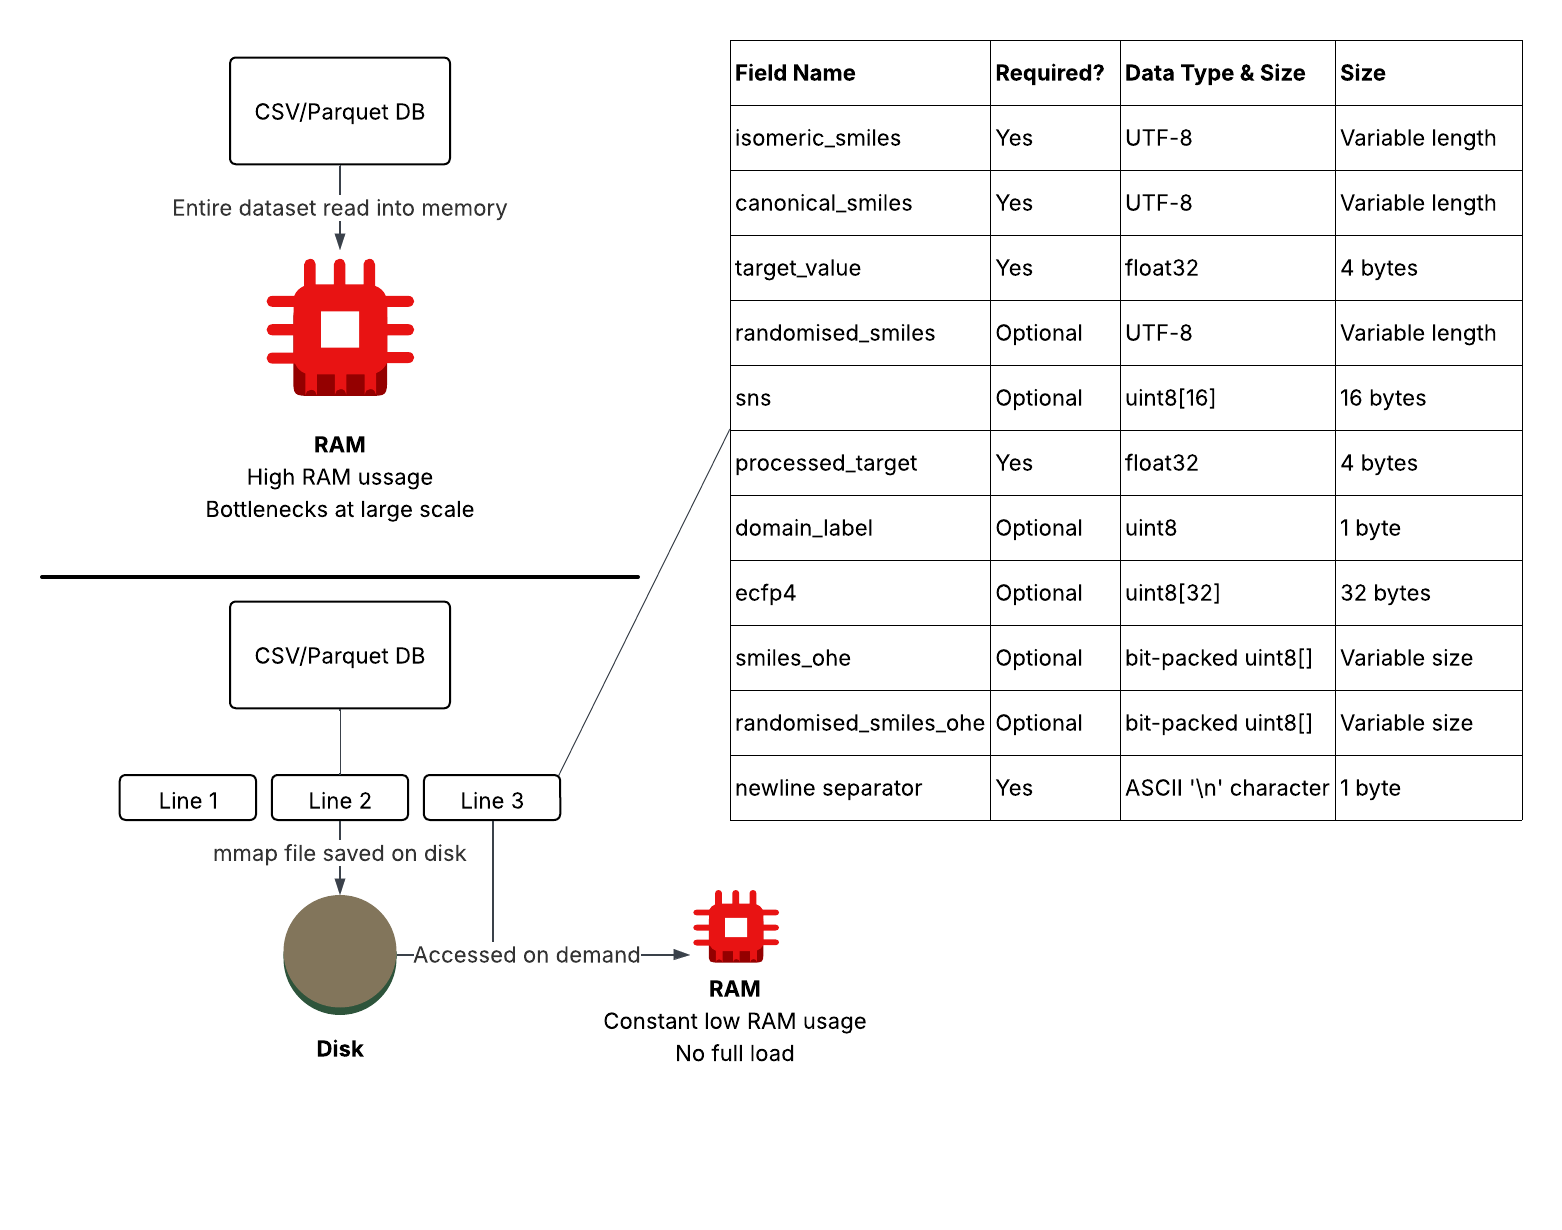
\includegraphics[width=0.95\textwidth,height=0.72\textheight,keepaspectratio]{figure_mmap_structure.png}
    \caption[In-memory and memory-mapped data loading.]{In-memory (top left) and memory-mapped (bottom left) data loading. Memory-mapped loading keeps each molecule as one record of a binary file on disk and reads records into memory on demand. The table on the right lists the fields of one record.}
    \label{fig:fig_mmap}
\end{figure}


\subsection{Uncertainty}
% [notes moved to thesis_notes_moved.md]

Up to this point we have been concerned with how noise affects the predictive performance of QSAR models. However, label noise should also affect the uncertainty these models report. Some models return only a point prediction, while others also return an estimate of uncertainty, either as a predicted distribution or as the spread across an ensemble. Furthermore, some report a single value of uncertainty while others report one that can be decomposed into an aleatoric and an epistemic component \citep{kendall2017}. The aleatoric component describes underlying noise the model associates with the data, while the epistemic component represents the uncertainty within the model's fit. We sought to determine if, as expected, the aleatoric component rises with injected label noise while the epistemic component does not.

For the BNN and VBLL transformations, we took the two components over $T = 100$ stochastic forward
passes \citep{kendall2017}:
\begin{equation}
\hat{u}^2_{\text{ale}}(x) = \frac{1}{T}\sum_{t=1}^{T}\hat{v}_t(x),
\qquad
\hat{u}^2_{\text{epi}}(x) = \frac{1}{T}\sum_{t=1}^{T}\big(\hat{\mu}_t(x) - \bar{\mu}(x)\big)^2 ,
\label{eq:sampling_split}
\end{equation}
where $\hat{\mu}_t(x)$ and $\hat{v}_t(x)$ are the mean and the variance returned for molecule $x$ on
pass $t$, and $\bar{\mu}(x)$ is the mean over passes. Here $\hat{v}_t(x)$ is the predicted observation
noise variance. It varies per molecule in the variance-head and heteroscedastic variants, and is one
number for the whole fit in the VBLL transformation. A full-BNN without a variance head returns no
variance, so its uncertainty is epistemic alone.

% TODO: review, needs manual review
The other models follow the same split. For GPs, the epistemic component is the posterior variance of the latent function and the aleatoric component is the learned observation noise \citep{Rasmussen2005}. Every GP except the heteroscedastic variant learns a single observation-noise variance for the whole fit, so its aleatoric component does not vary between molecules. For QRF models, each leaf holds several training molecules, and the aleatoric component for a molecule is the variance of the training labels in the leaf it falls into, averaged over the trees. The epistemic component is the variance of the leaf means across the trees. NGBoost predicts one variance for each molecule from a single fit, which is aleatoric alone \citep{Duan2020}. In every model, the total uncertainty is the sum of the aleatoric and epistemic components.

No held-out label carries injected noise, so every comparison against the injected noise was made on
training molecules. Each training set was divided into five folds grouped on Murcko scaffolds, and each
molecule was scored by a refit that excluded its own fold. For NGBoost on QM9, three of the five folds
were scored to limit its cost. No uncertainty was calibrated after fitting.


\subsection{Evaluation}
% [notes moved to thesis_notes_moved.md]
We computed statistics on the held-out molecules: for QM9 the test split, and for the three assay datasets the held-out fold of the scaffold cross-validation. Different combinations of dataset, model, representation, noise condition, and noise level are examined in each scenario. We used the coefficient of determination ($R^2$) throughout. For molecule $i$, let $y_i$ be the clean label, $\hat{y}_i$ the prediction, $\epsilon_i$ the noise injected into its label and $u_i$ the predicted uncertainty.

% TODO: review, needs manual review
To evaluate the effect of label noise, we tracked predictive performance retention under increasing artificial noise. For each QSAR pairing we recorded $R^2(x)$ at each noise level $x$, and normalized it to obtain the retention ratio $R^2(x)/R^2(0)$. To quantify robustness, we used the normalized area under this retention curve, \aucnorm{} (Equation~\ref{eq:auc_norm}), evaluated using the trapezoidal rule over the seven noise levels, $x \in \{0, 0.2, 0.3, 0.5, 0.75, 1.0, 1.5\}$, in the units of Equation~\ref{eq:dose_matching}. For censoring, the area is taken over the fractions of labels clipped, from 0 to 0.5, so its \aucnorm{} is not on the same axis as the other conditions.

An \aucnorm{} value near 1 indicates that the QSAR model in question has retained predictive performance with artificial noise, meaning it is more robust to noise. Since we normalize the curve by its own clean-label predictive performance, a model with a low clean $R^2$ has less to lose, so \aucnorm{} is reported beside clean $R^2$. We excluded every QM9 replicate or scaffold fold with a clean $R^2 < 0.3$ from the robustness analysis (Additional file~\ref{app:noise:sec:excluded_configurations}), as performance retention ratios become unstable when the clean-label denominator approaches zero. On QM9 one \aucnorm{} is computed per replicate, and we report the median over the 10 replicates. On the three assay datasets one value is computed per scaffold fold, and the median over the five folds is reported. 

% TODO: review, needs manual review
To test whether a model's robustness follows from its clean predictive performance, we computed Spearman's rank correlation ($\rho$) between clean $R^2$ and \aucnorm{} across the thirteen base models.

We conducted a separate analysis of variance (ANOVA) for each noise condition to identify the
relative contributions of molecular representation and model architecture to both predictive
performance and noise robustness. For a given metric $y$, either $R^2$ at a noise level of 1.0 (0.75 on Caco-2) or
\aucnorm:
\begin{equation}
y_{fmjr} = \mu + s_r + \alpha_f + \gamma_{m(f)} + \beta_j + (\alpha\beta)_{fj} + (\gamma\beta)_{m(f)j} + e_{fmjr},
\end{equation}
where $s_r$ represents the effect of replicate $r$, $\alpha_f$ represents the effect of model family $f$, $\gamma_{m(f)}$ represents the effect of model architecture $m$ within its family, $\beta_j$ represents the effect of
molecular representation $j$, $(\alpha\beta)_{fj}$ and $(\gamma\beta)_{m(f)j}$ are the interaction terms, and $e_{fmjr}$ is the
residual. The proportion of variance explained by each term was calculated as the
effect size
\begin{equation}
\eta^2_{\text{term}} = \frac{SS_{\text{term}}}{SS_{\text{total}}},
\end{equation}
using Type I (sequential) sums of squares, entered in the order replicate, model family, model architecture within family, molecular
representation, interaction. The 10 QM9 replicates provide the residual; on the three assay datasets the five scaffold folds take the place of the replicates. The uncertainty on each share is the 95\% interval of $\eta^2$ over 1,000 bootstrap resamples of whole replicates. These shares describe the models and representations tested here, not the choice of model or representation in general. 

ANOVA relies on the assumption that observations both within and across groups are independent. Two features of this study break that assumption. First, each QM9 replicate uses the same data split and the same noise draw for every model and representation, so observations from one replicate are not independent of each other; we therefore entered the replicate as a block. Second, across the whole set of models in this study, some pairs produced similar predictions that are not independent, so a method present in several near-identical versions would count several times toward the share of model architecture. To handle this issue, we grouped the models into families. We considered grouping pairs of models that share a method or an architecture, and compared each pair on clean $R^2$ and on \aucnorm{} under the three noise conditions run on every representation, separately on each of the six representations, which gives 24 comparisons per pair. A pair was grouped when the mean difference between the two models was smaller than their standard deviation across replicates in at least two thirds of these comparisons (Additional file~\ref{app:noise:sec:model_redundancy}). Five families met this criterion: RF with QRF (16 of 24), XGBoost with LightGBM (23 of 24), NN-$\alpha$ with BNN-$\alpha$ (20 of 24), NN-$\beta$ with BNN-$\beta$ (18 of 24), and VBLL-$\alpha$ with VBLL-$\beta$ (20 of 24). VBLL did not group with the plain or Bayesian network of its own architecture (4 to 10 of 24), as its clean $R^2$ was lower by 0.02 to 0.09, and NGBoost did not group with XGBoost or LightGBM (2 and 3 of 24). The two architectures of the plain networks, and of the Bayesian networks, also met the criterion (18 and 17 of 24); we grouped by architecture instead, which the evidence supports equally well. The thirteen base models therefore form eight families. Within these families, the differences between models accounted for at most 1.0\% of the variance in any outcome and noise condition on QM9, and up to 15.1\% of predictive performance on clean labels on the three assay datasets. We also ran Tukey's honestly significant difference test between the members of each family, separately for each representation (Additional file~\ref{app:noise:sec:tukey_within_families}). With 10 replicates it detects differences smaller than the variation between replicates, so we report it beside the size of each difference rather than use it to form the families.

% TODO: review, needs manual review
Across representations, we considered grouping Sort \& Slice with the ECFP4 fingerprint, as both encode overlapping circular substructure information. The grouping criterion held for none of the 13 base models on clean $R^2$, so all six representations were kept as separate levels (Additional file~\ref{app:noise:sec:representation_redundancy}).

% TODO: review, needs manual review
To assess the interaction between uncertainty estimation and label noise, we carried out four analyses. The first tested whether uncertainty rises with label noise, as measured by the mean $u_i$ over held-out molecules at the highest noise level
divided by its value with no added noise, in each fold. The second pertains to models that report separate aleatoric and epistemic components. We divided the increase of mean epistemic uncertainty between the highest level of noise and clean labels by the increase in the mean aleatoric component to determine how each responds to label noise. A ratio near 0 means the added noise was attributed to the labels while a ratio of 1 or above means the epistemic component grew as much or more. We also compared the mean aleatoric component with the standard deviation of the injected noise. The third tested whether per-sample uncertainty values track injected label noise, as measured by the Spearman correlation between $u_i$ and $|\epsilon_i|$ over out-of-fold training molecules, per fold and per noise level. We also report the Spearman correlation between $u_i$ and the absolute error of the prediction. The fourth tested whether dividing a molecule's out-of-fold absolute error by $u_i$ ranks the corrupted labels better than the error alone, and we report the difference between the two Spearman correlations with $|\epsilon_i|$.


